\section{Dynamic Link and Clustering Validation}
\label{sec:dynamic_link_clustering_validation}

\subsection{Dynamic Trial Configuration}

Three corrected dynamic trials were included in this comparison. Each run lasted approximately 70~s and recorded the movement, link metrics and cluster assignments for the three UAVs. The older original Trial~1 was excluded because it was not directly comparable with the corrected runs. Under the canonical counting rule, the first 0.01~s of clustering initialization and its assignment states were removed. This left 35 complete assignment states per trial.

Table~\ref{tab:dynamic_trial_summary} gives the retained trial-level clustering results. The first retained state formed the baseline, so it was not counted as a transition.

\begin{table}[htbp]
    \centering
    \small
    \caption{Canonical clustering results for the three corrected dynamic trials.}
    \label{tab:dynamic_trial_summary}
    \begin{tabular}{lrrrrrr}
        \toprule
        Trial & Duration (s) & States & Primary & Retention (\%) & Primary changes & Backup changes \\
        \midrule
        Trial 1 & 69.842 & 35 & UAV3 & 100 & 0 & 2 \\
        Trial 2 & 69.800 & 35 & UAV3 & 100 & 0 & 4 \\
        Trial 3 & 69.781 & 35 & UAV1 & 100 & 0 & 3 \\
        \bottomrule
    \end{tabular}
\end{table}

\subsection{Link-Quality Variation during UAV Movement}

The recorded network-link data were summarised at trial level rather than treating every link row as a separate experiment. Table~\ref{tab:dynamic_link_quality} compares the mean RSSI, SNR and obstacle loss. By RSSI and SNR, average link quality was strongest in Trial~1. Trial~3 had the weakest mean RSSI and SNR, together with the highest mean obstacle loss.

\begin{table}[htbp]
    \centering
    \caption{Mean dynamic link-quality measurements for each corrected trial.}
    \label{tab:dynamic_link_quality}
    \begin{tabular}{lrrr}
        \toprule
        Trial & Mean RSSI (dBm) & Mean SNR (dB) & Mean obstacle loss (dB) \\
        \midrule
        Trial 1 & -58.770 & 35.230 & 2.072 \\
        Trial 2 & -59.516 & 34.484 & 1.854 \\
        Trial 3 & -62.373 & 31.627 & 2.705 \\
        \bottomrule
    \end{tabular}
\end{table}

\begin{figure}[htbp]
    \centering
    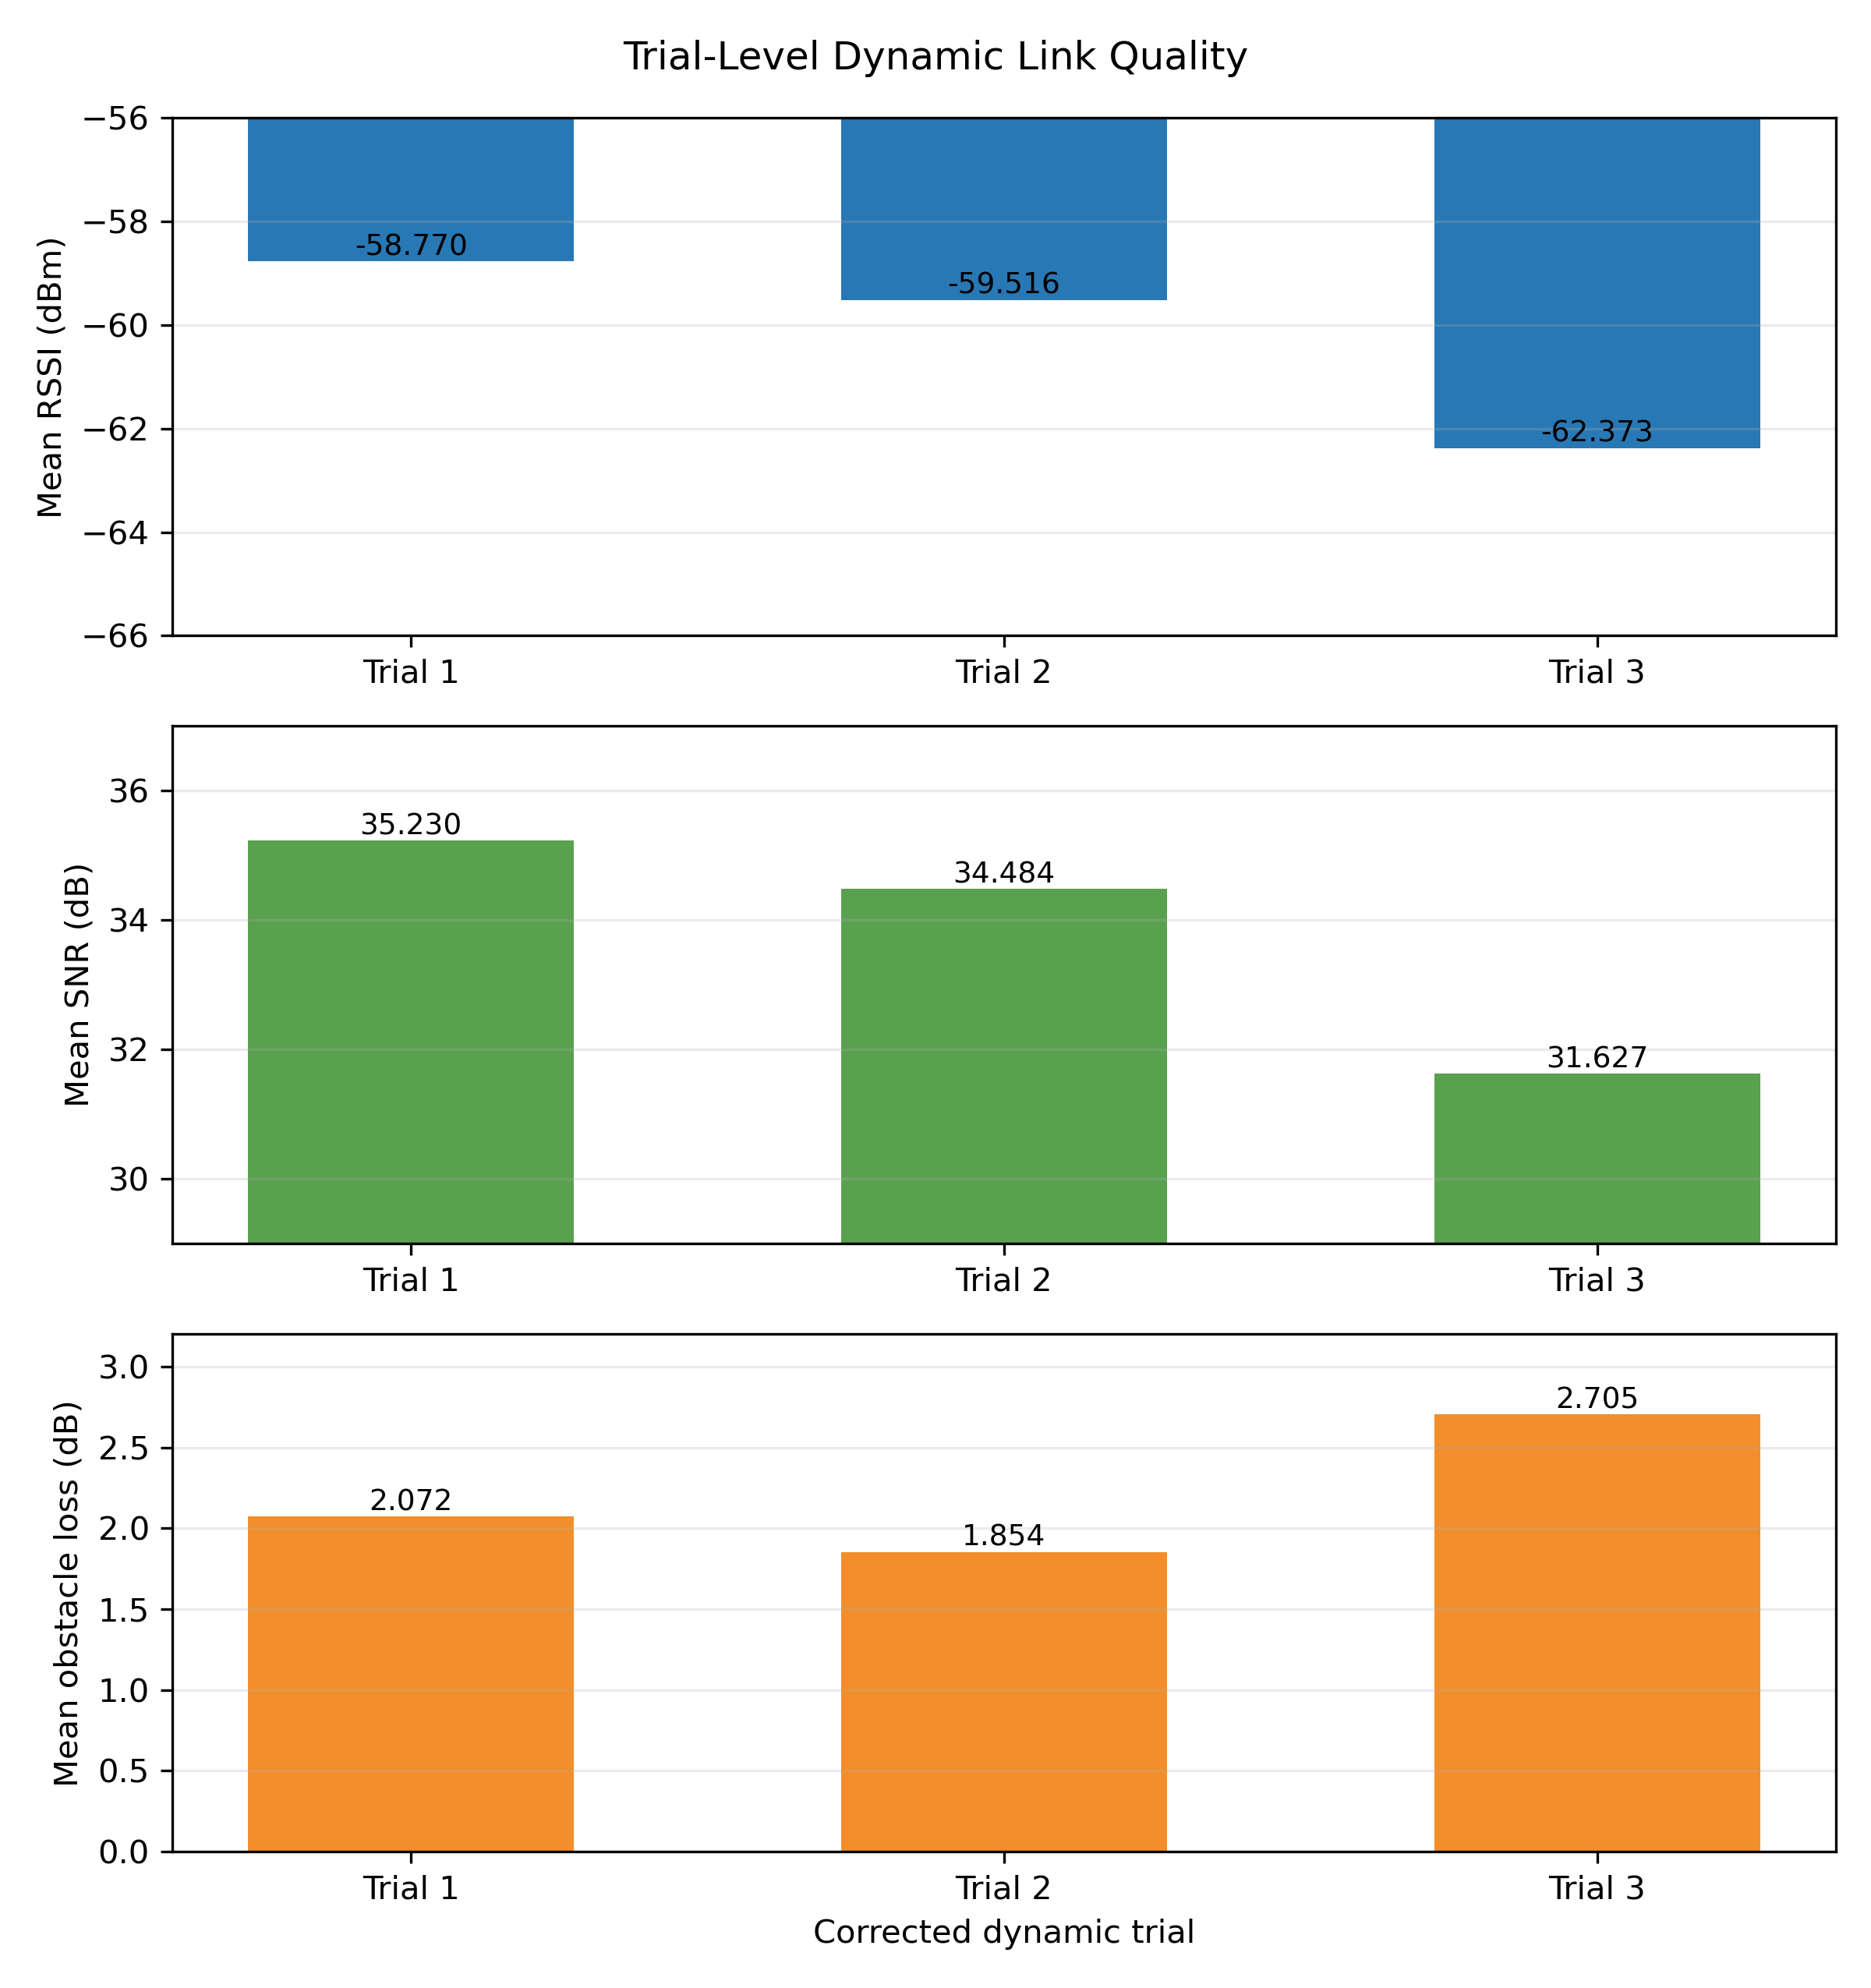
\includegraphics[width=0.82\textwidth]{images/chapter5/clustering/link_quality_by_trial.png}
    \caption{Trial-level mean RSSI, SNR and obstacle loss for the corrected dynamic runs.}
    \label{fig:link_quality_by_trial}
\end{figure}

Mean values do not show every temporary degradation. Figure~\ref{fig:representative_rssi_timeline} therefore plots the corrected Trial~1 RSSI samples for GCS-to-UAV links only. Short, severe RSSI drops occurred during movement, but they should not be called physical outages without matching packet-delivery evidence.

\begin{figure}[htbp]
    \centering
    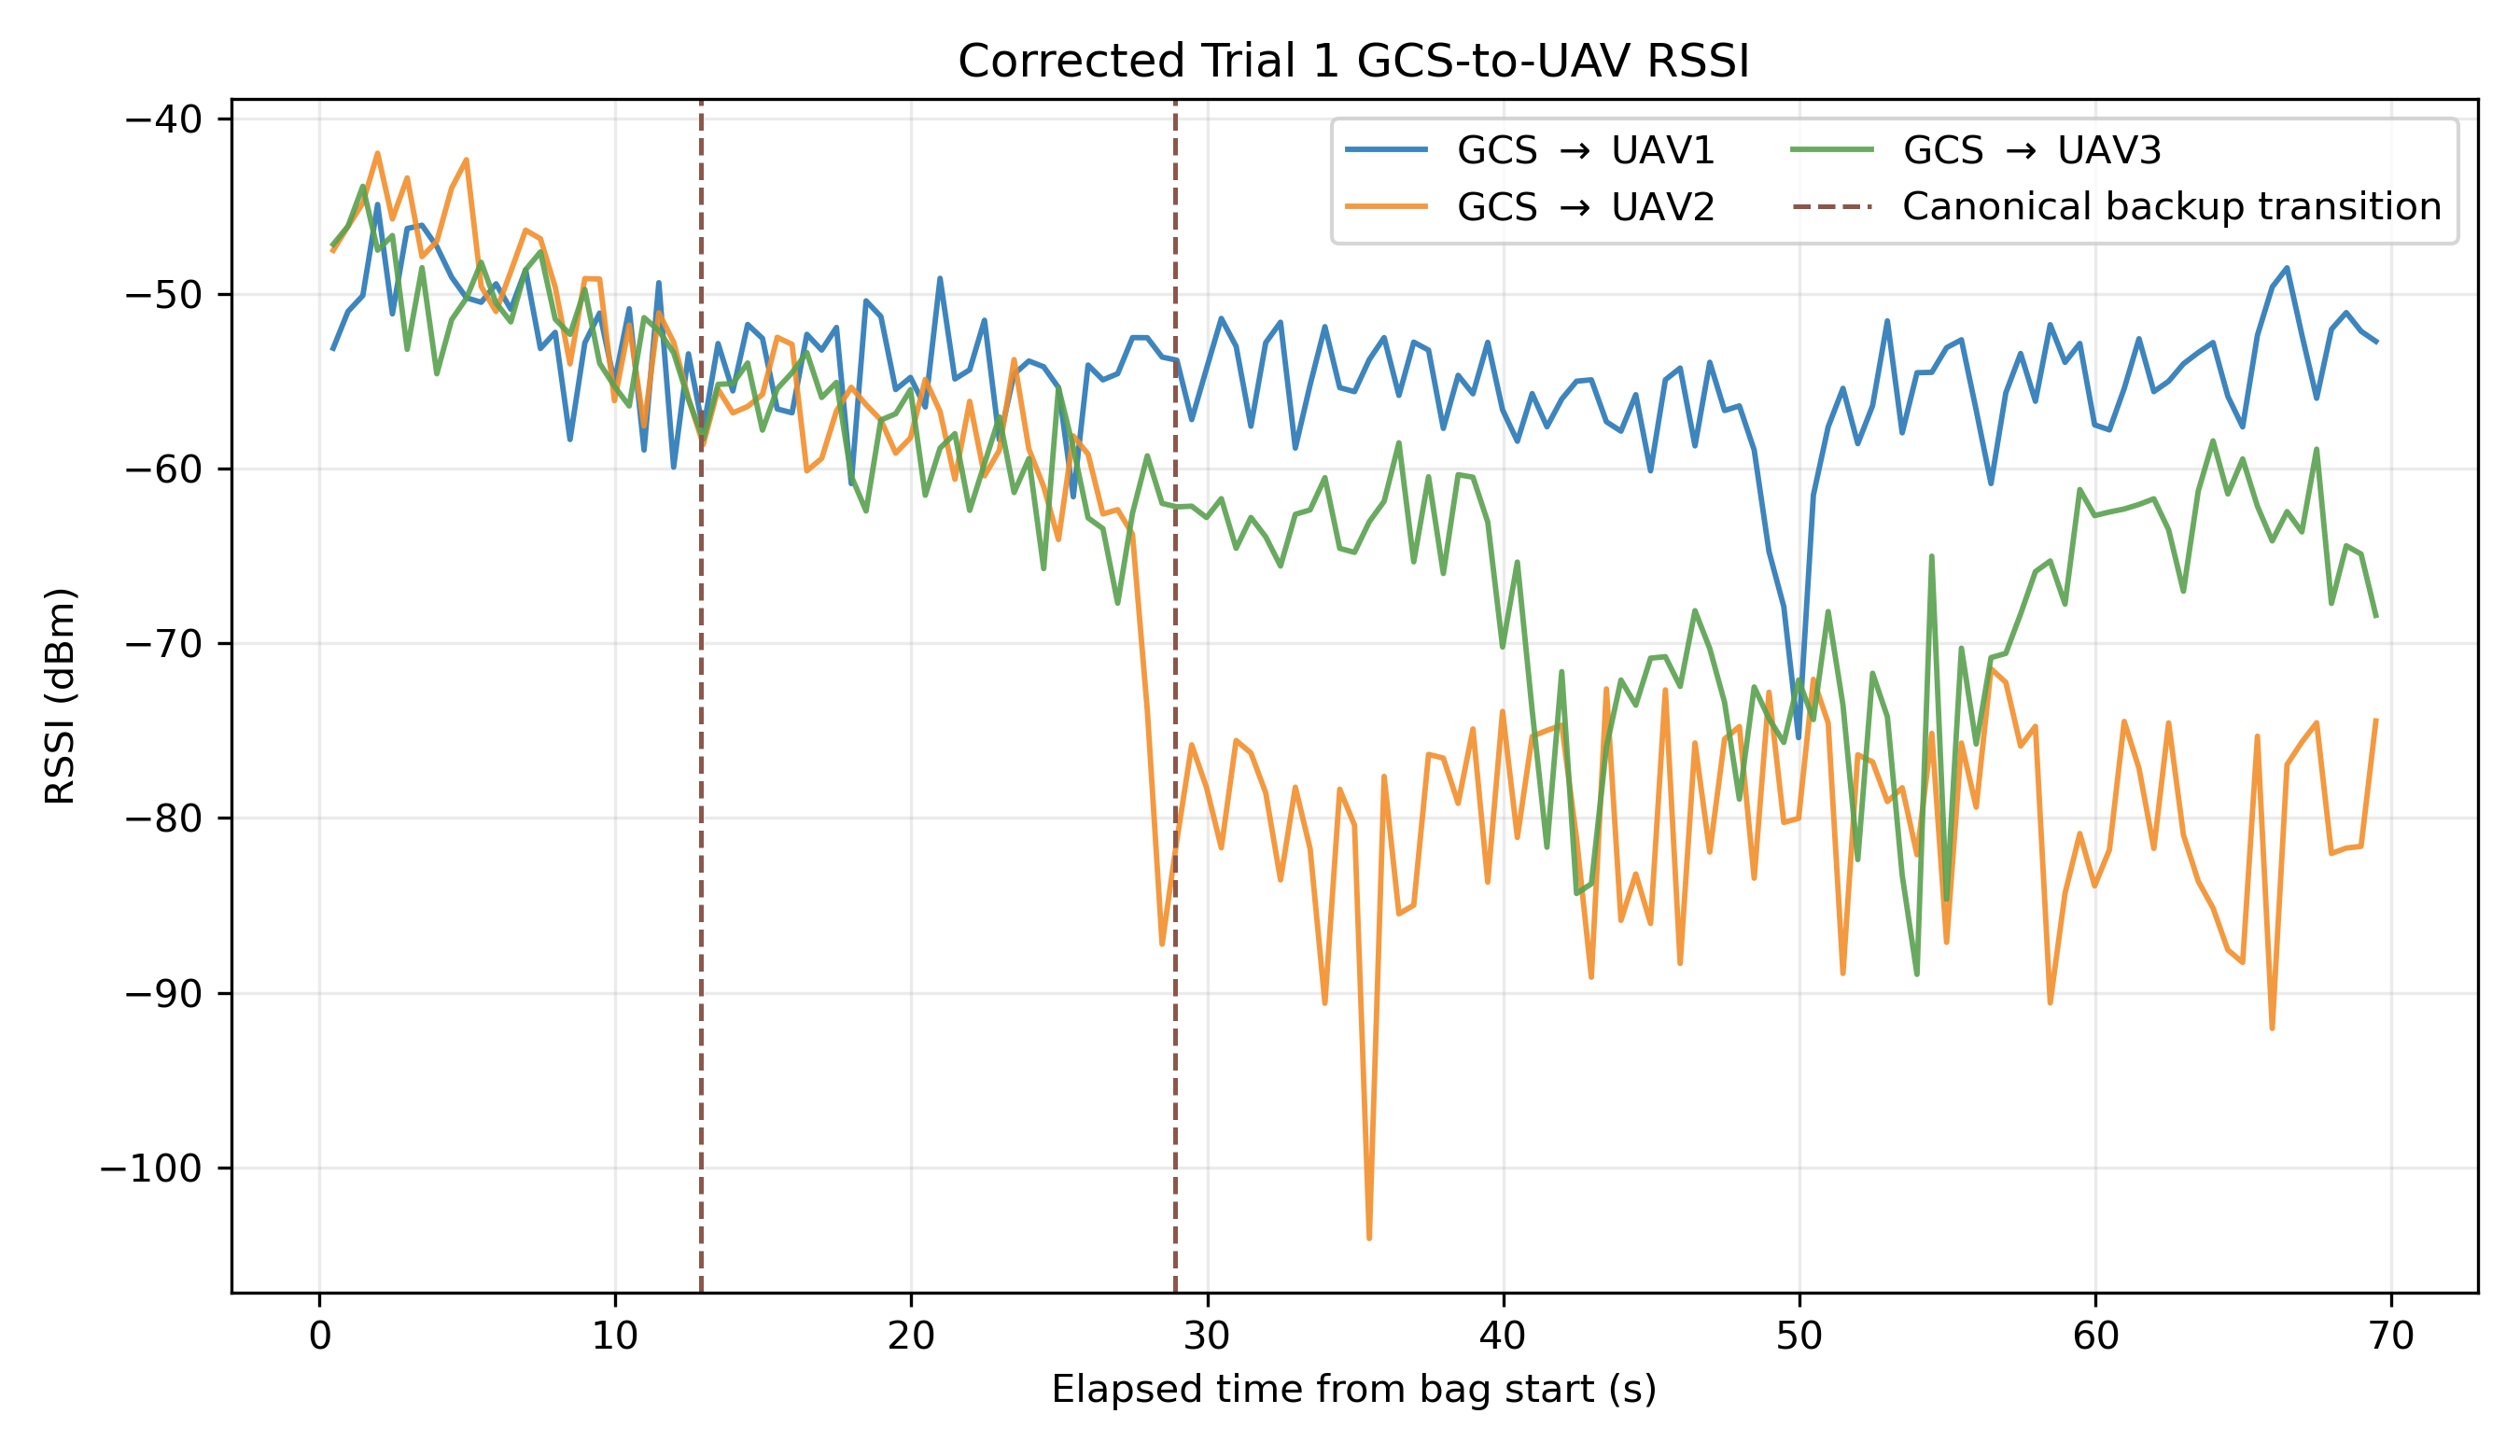
\includegraphics[width=0.88\textwidth]{images/chapter5/clustering/representative_rssi_timeline.png}
    \caption{GCS-to-UAV RSSI during corrected Trial 1, with canonical backup transitions marked.}
    \label{fig:representative_rssi_timeline}
\end{figure}

Figure~\ref{fig:representative_topology} provides a second view of the movement. It uses the first and last canonically retained Trial~1 assignments, matched to the nearest recorded position timestamp. Only node positions and recorded cluster roles are shown; no direct communication links were inferred.

\begin{figure}[htbp]
    \centering
    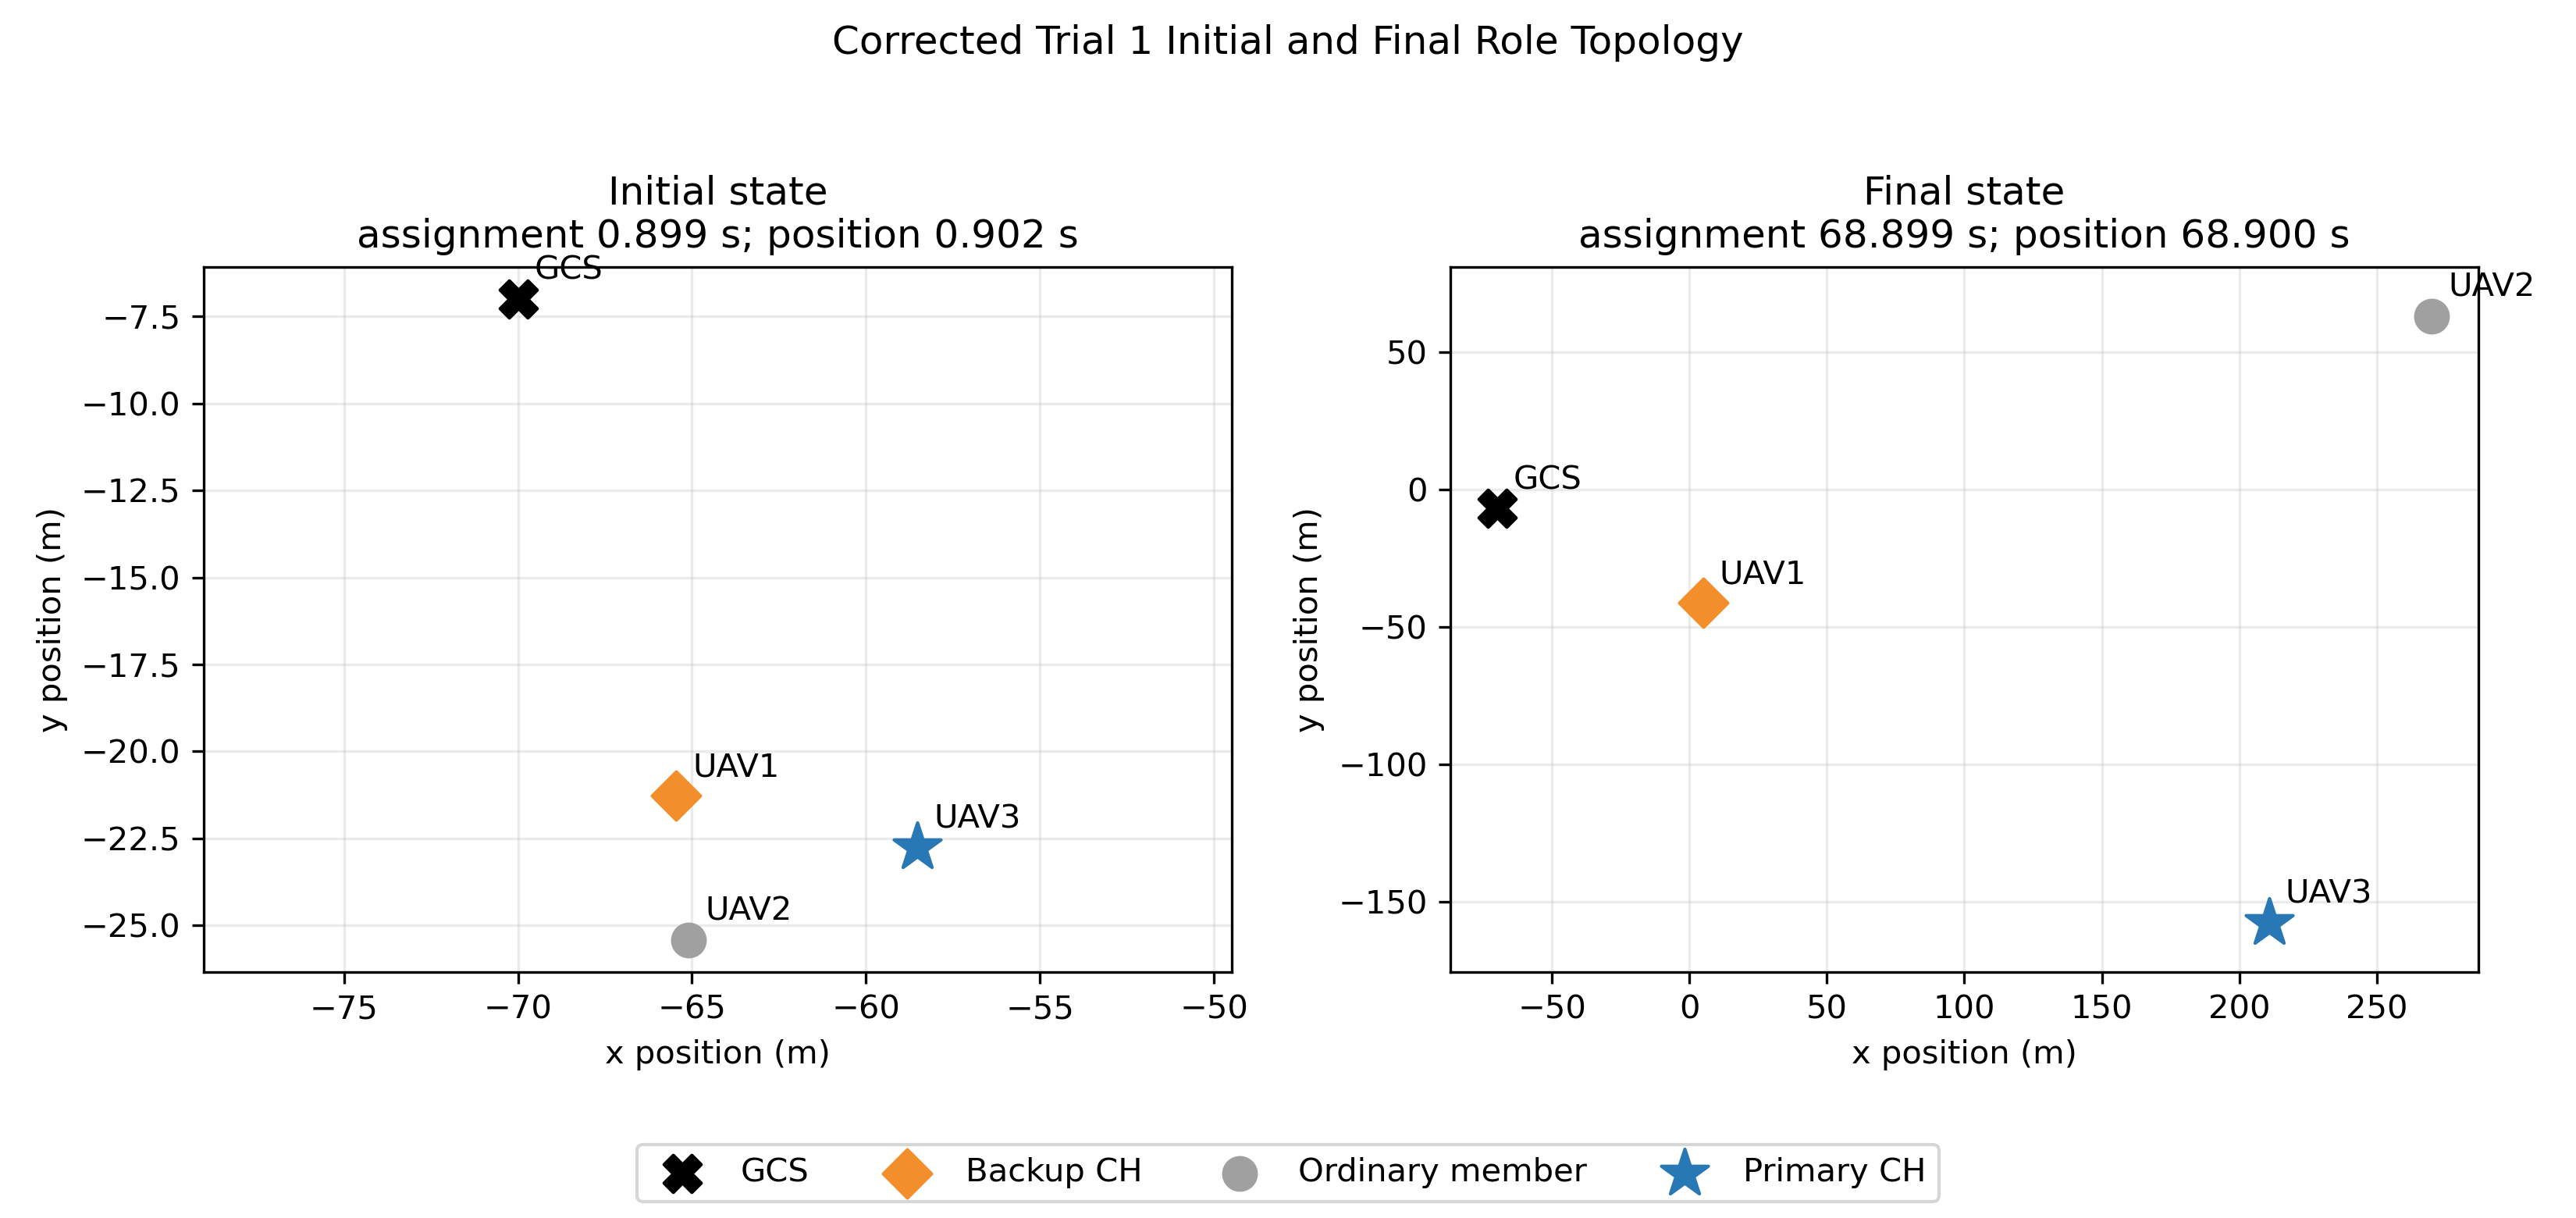
\includegraphics[width=0.92\textwidth]{images/chapter5/clustering/representative_topology_initial_final.png}
    \caption{Initial and final corrected Trial 1 positions and cluster roles.}
    \label{fig:representative_topology}
\end{figure}

\subsection{Primary Cluster-Head Stability}

UAV3 remained primary throughout Trials~1 and 2, while UAV1 remained primary throughout Trial~3. Retention was 100\% in every run and there were no canonical primary transitions. The experiments demonstrated stable primary leadership under the recorded mobility conditions. Since no primary change occurred, primary switching was not experimentally validated.

\subsection{Backup Cluster-Head Reselection}

The backup role changed twice in Trial~1, four times in Trial~2 and three times in Trial~3. Figure~\ref{fig:cluster_roles_timeline} shows these changes alongside the constant primary role. Transitions were counted from changes between complete assignment states after the initialization interval. Repeated event publications were not counted separately, and initialization messages were excluded. The event totals and canonical role-transition counts therefore differ.

\begin{figure}[htbp]
    \centering
    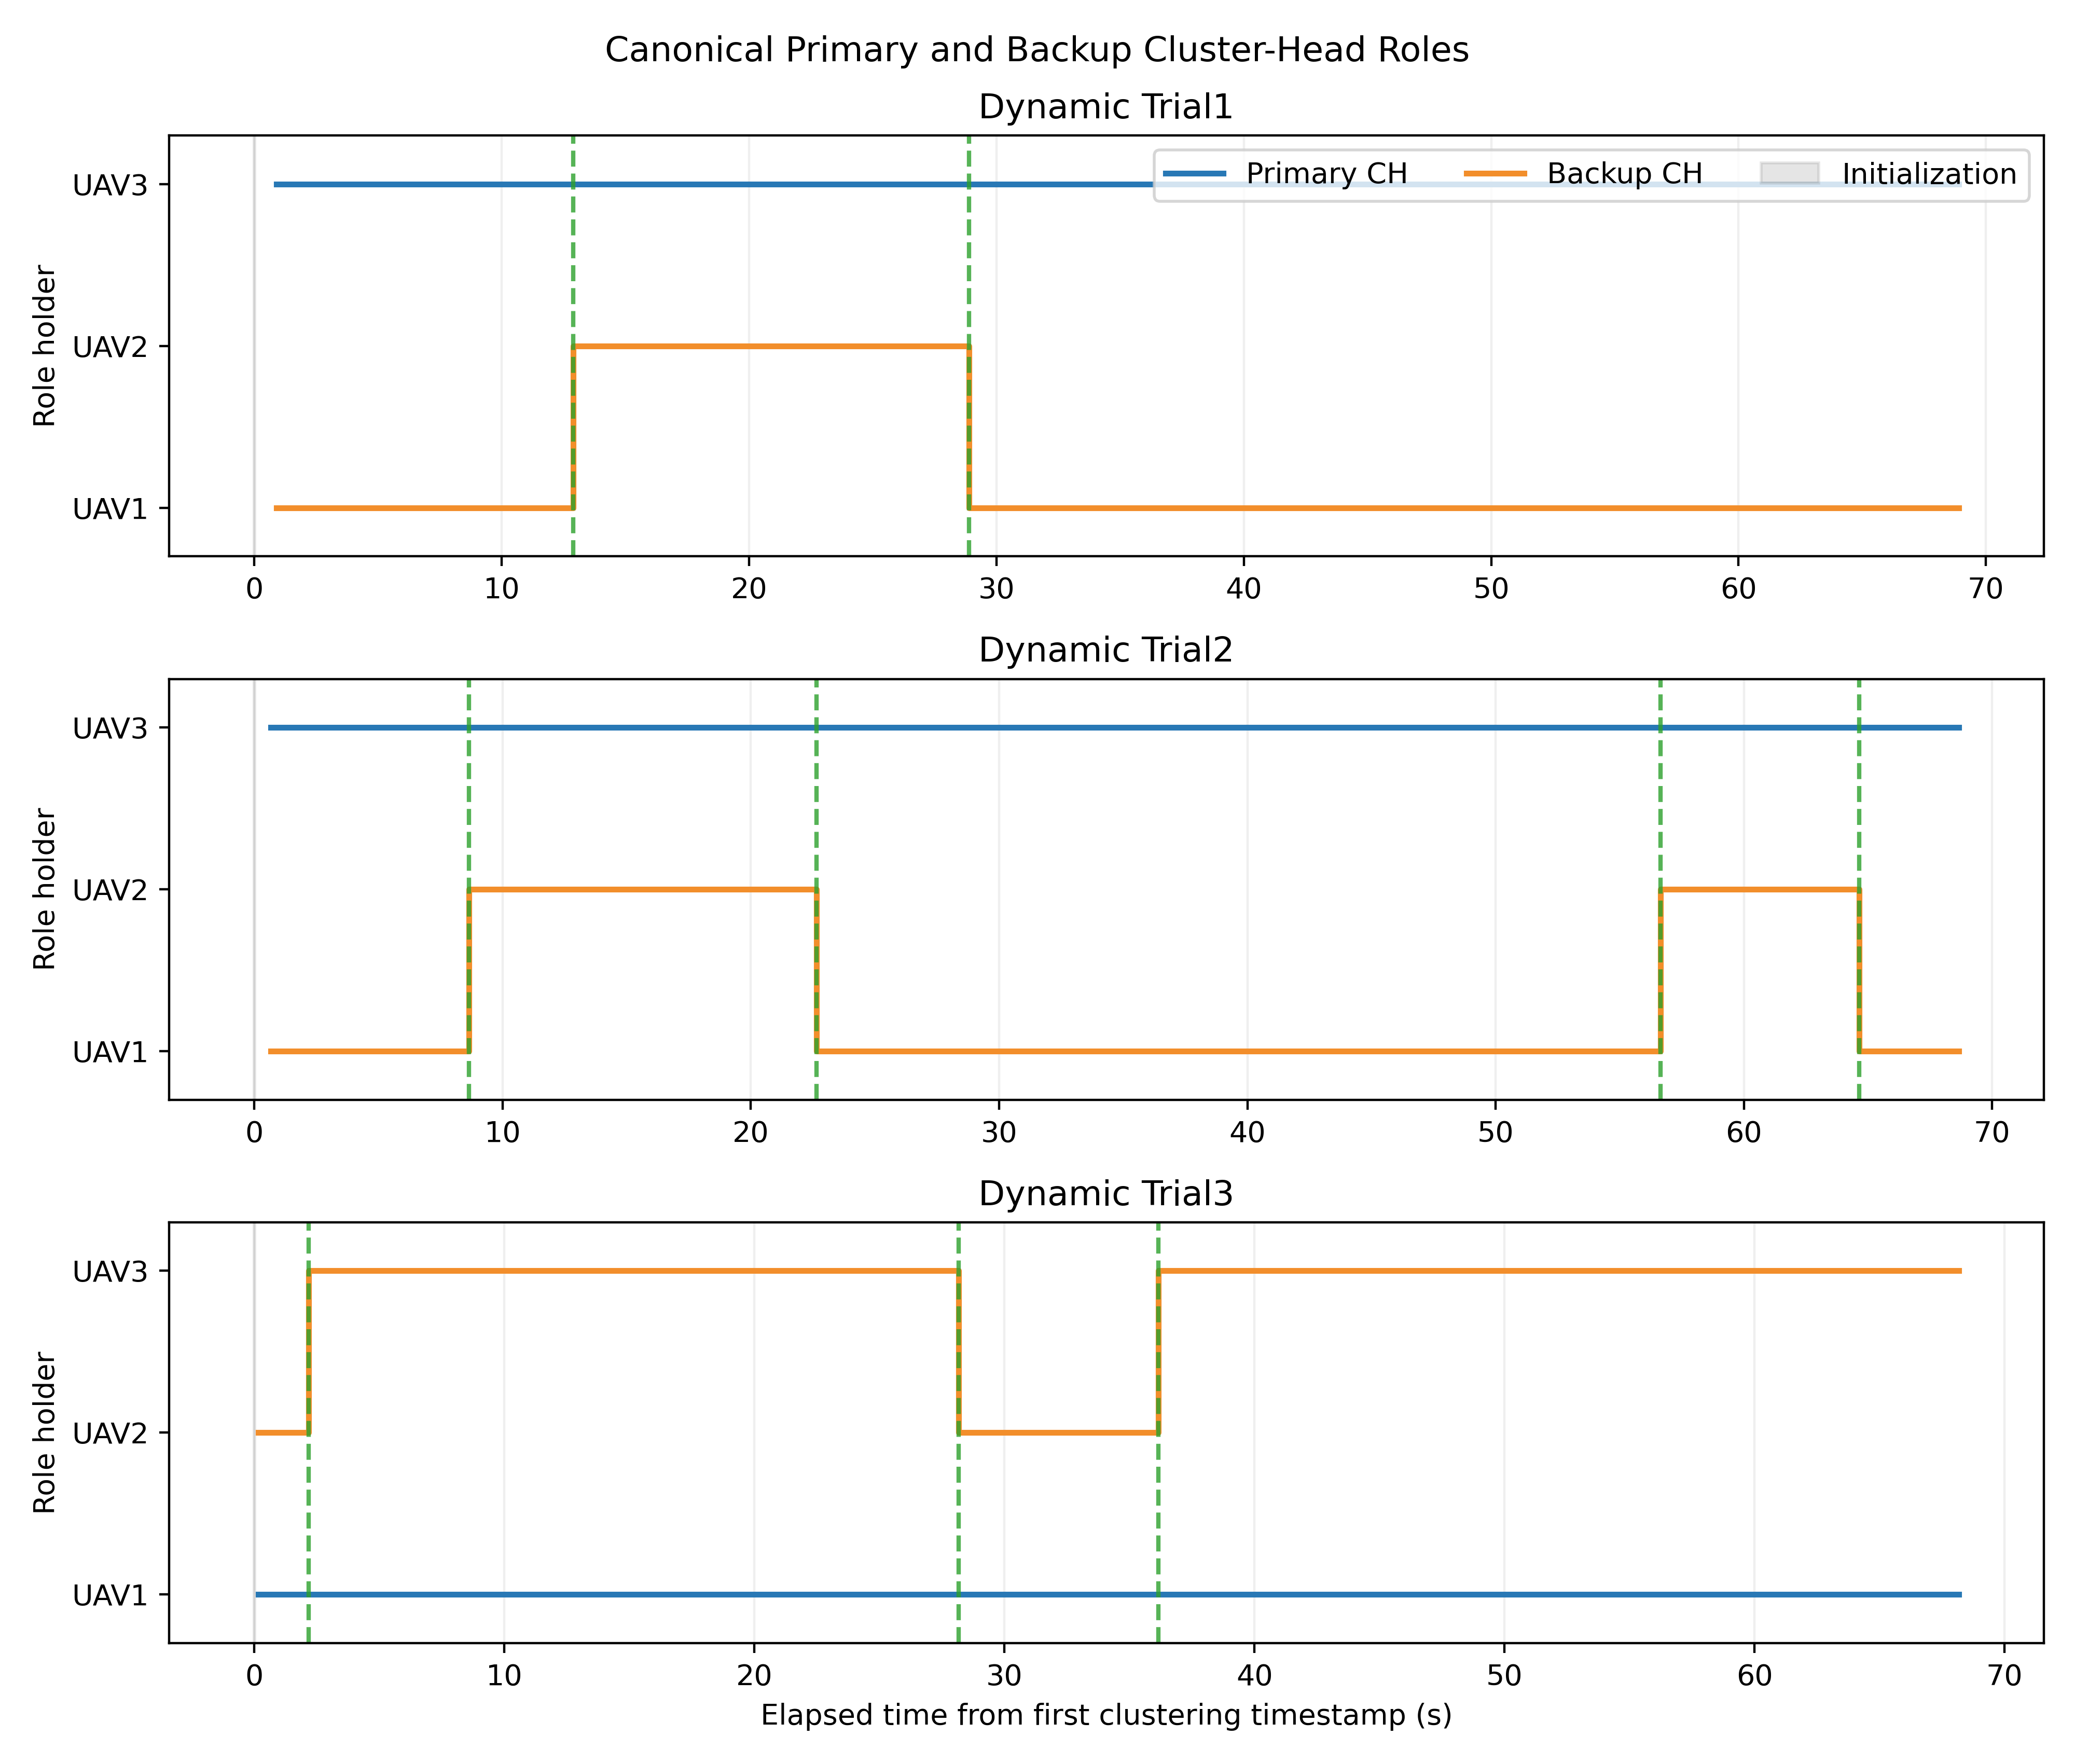
\includegraphics[width=0.92\textwidth]{images/chapter5/clustering/cluster_roles_timeline.png}
    \caption{Canonical primary and backup cluster-head roles across the corrected trials. Dashed markers show counted backup transitions.}
    \label{fig:cluster_roles_timeline}
\end{figure}

\subsection{Implementation and Validation Scope}

Controlled primary switching used score-margin, consecutive-win and holding-time logic. This path existed in the contemporaneous clustering implementation, but it was not triggered during the corrected dynamic trials. The recorded results therefore validate primary stability rather than handover behaviour.

A threshold-driven primary-link-failure path also existed and selected the best eligible candidate. It did not guarantee immediate promotion of the stored backup. No dedicated emergency-failover test was found, so emergency failover and its recovery time were not experimentally validated.

\subsection{Clustering Validation Summary}

The corrected trials produced dynamic position, RSSI, SNR and obstacle-loss measurements together with complete clustering states. Primary selection remained stable, while backup reselection occurred in every run. Controlled handover and emergency failover remain outside the validated experimental scope and require separate targeted tests before fault-tolerance claims can be made.
